\documentclass[a4paper]{article}
\usepackage[T1]{fontenc}
\usepackage[english]{babel}
\usepackage{clrscode4e} % Algorithm template from Introduction to Algorithms 4th
\usepackage[left=2cm,right=2cm,top=1cm,bottom=2cm]{geometry} % page settings
\usepackage{amsthm, amsmath} % provides many mathematical environments & tools
\usepackage{tikz} % draw pictures
\usepackage{tabularray}
\usepackage[noend]{algorithmic}
\usepackage{tabularx}
\usepackage[noend]{algorithmic}
\usepackage{algorithm}
\usepackage{arydshln}
\usepackage{forest}
\usepackage{adjustbox}

%-----------------------------------------------------------
% Custom commands
%-----------------------------------------------------------
\usetikzlibrary{positioning,matrix, arrows.meta}
\tikzset{box/.style={draw, thick, minimum width=1cm, minimum height=1cm}}

\newenvironment{solution}
  {\begin{proof}[Solution]}
  {\end{proof}}
\renewcommand{\qedsymbol}{\rule{0.7em}{0.7em}}

\makeatletter
\renewenvironment{proof}[1][\proofname]{%
  \par\pushQED{\qed}\normalfont%
  \topsep6\p@\@plus6\p@\relax
  \trivlist\item[\hskip\labelsep\bfseries#1\@addpunct{.}]%
  \ignorespaces
}{%
  \popQED\endtrivlist\@endpefalse
}
\makeatother

\tikzset{
      heap/.style={
        every node/.style={circle,draw,minimum width=8mm},
        level 1/.style={sibling distance=80mm},
        level 2/.style={sibling distance=50mm},
        level 3/.style={sibling distance=20mm}, % <----- Here's the lowest level of your tree
        level 4/.style={sibling distance=10mm}
      }
    }

\setlength{\parindent}{0mm}

%-----------------------------------------------------------
% Document
%-----------------------------------------------------------
\begin{document}

\title{Algorithms: Homework 1}
\author{Li-Yuan Wei}
\date{\today}
\maketitle

\subsection*{Problem 1}
Consider the following selection sort algorithm: finding the smallest element and exchanging it with $A[1]$, and then finding the second smallest element and exchanging it with $A[2]$. Continue in this manner for the first $n-$1 elements of $A$. What are the best-case running time and worst-case running time for this algorithm? Simulate what we did for insertion sort to give your conclusion.
\begin{solution}
Psuedocode for selection sort: \\
\noindent
  \begin{tabularx}{\textwidth}{>{\footnotesize}rXcc@{}}
    \\[-1.5ex] \hline
    \multicolumn{2}{@{}l}{\refstepcounter{algorithm}\label{selection} $\proc{Selection-Sort}(A,n)$} & Cost & Times \\
    \hline
     1: & \For $i \gets 1$ \To $\attrib{A}{length} -1$ & c1 & $n$ \\
     2: & \quad \textbf{min} $\gets i$ & c2 & $n - 1$ \\
     3: & \quad \For $j \gets i + 1$ \To $\attrib{A}{length}$ & c3 & $\sum_{j = 2}^{n}(t_j)$\\
     4: & \quad\quad \If $A[j] < $A[\textbf{min}$]$ & c4 & $\sum_{j = 2}^{n}(t_j - 1)$ \\
     5: & \quad\quad\quad \textbf{min} $\gets j$ & c5 & $\sum_{j = 2}^{n}(t_j - 1)$ \\
     6: & \quad \If $i \neq \textbf{min}$ & c6 & $n - 1$\\
     7: & \quad\quad exchange $A[i]$ with $A[\textbf{min}]$ & c7 & $n - 1$ \\
\hline
  \\ [-0.2cm]
  \end{tabularx}

  The total running time of selection sort is:

  \begin{align*}
    T(n) &= c_1 n + c_2(n - 1) + c_3\sum_{j = 2}^{n}(t_j) +c_4\sum_{j = 2}^{n}(t_j - 1) + c_5\sum_{j = 2}^{n}(t_j - 1) + c_6(n - 1) + c_7(n - 1) \\
  \end{align*}

  We first analyze the \textbf{best-case} running time of this algorithm. Let's assume the input array is a sorted sequence in increasing order. Every $A[i]$ we selected in line $2$ is already the smallest element in $A$. Thus, this algorithm will not execute line $5, 7$ under this condition. However, this algorithm will still iterate the whole sequence, which starts from index $j$, in line $3$ because it will need to check if $A[\textbf{min}]$ is the smallest element.
  \begin{align*}
    T(n)  &= c_1 n + c_2(n - 1) + c_3(\frac{n^2 + n}{2} - 1) + c_4(\frac{n^2 - n}{2}) + c_6(n -1)\\
         &= (\frac{c_3}{2} + \frac{c_4}{2}) n^2 + (c_1 + c_2 + \frac{c_3}{2} - \frac{c_4}{2} + c_6)n - (c_2 + c_6) \\
  \end{align*}

  We conclude the \textbf{best-case} running time for selection sort is $\Theta(n^2)$ since $n^2$ is the dominant term in $T(n)$. \qed

  Additionally, we assume the input array as a decreasing sorted sequence. This is the worst-case scenario because the program will execute line $5$ whenever it compares $A[\textbf{min}]$ with $A[j]$ in line $4$, and executes exchange in line $7$.
  \begin{align*}
    T(n) &=c_1 n + c_2(n - 1) + c_3(\frac{n^2 + n}{2} - 1) + c_4(\frac{n^2 - n}{2})+c_5(\frac{n^2 - n}{2}) + c_6(n - 1) + c_7(n - 1)\\
         &= (\frac{c_3}{2} + \frac{c_4}{2} + \frac{c_5}{2})n^2 + (c_1 + c_2 + \frac{c_3}{2} - \frac{c_4}{2} - \frac{c_5}{2} + c_6 + c_7)n - (c_2 + c_3 + c_6 + c_7)
  \end{align*}

  Therefore, we conclude that the \textbf{worst-case} running time for selection sort is still $\Theta(n^2)$.
\end{solution}

\subsection*{Problem 2}
What are the best-case running time and worst-case running time for bubblesort? Please refer to the following pseudo-code of bubblesort. Simulate what we did for insertion sort to give your conclusion.
\begin{solution}
Psuedocode for bubble sort: \\
\noindent
  \begin{tabularx}{\textwidth}{>{\footnotesize}rXcc@{}}
    \\[-1.5ex] \hline
    \multicolumn{2}{@{}l}{\refstepcounter{algorithm}\label{bubble} $\proc{Bubble-Sort}(A,n)$} & Cost & Times \\
    \hline
     1: & \For $i \gets 1$ \To $\attrib{A}{length} -1$ & c1 & $n$ \\
     2: & \quad \For $j \gets \attrib{A}{length}$ \Downto $i + 1$ & c2 & $\sum_{j = 2}^{n}(t_j)$\\
     3: & \quad\quad \If $A[j] < A[j - 1]$ & c3 & $\sum_{j = 2}^{n }(t_j - 1)$\\
     4: & \quad\quad\quad exchange $A[j]$ with $A[j - 1]$ & c4 & $\sum_{j = 2}^{n}(t_j - 1)$ \\
\hline
  \\ [-0.2cm]
  \end{tabularx}

  The total running time of bubble sort is:

  \begin{align*}
    T(n)  &= c_1 n + c_2\sum_{j = 2}^{n}(t_j) + c_3\sum_{j = 2}^{n }(t_j - 1) + c_4\sum_{j = 2}^{n}(t_j - 1) \\
  \end{align*}

  For the \textbf{best-case} running time, we assume the input is a sorted sequence in increasing order. Therefore, $t_j = 1$ in line $4$ because there will need no exchange.

  \begin{align*}
    T(n)  &= c_1 n + c_2(\frac{n^2 + n}{2} - 1) + c_3(\frac{n^2 - n}{2}) \\
          &= (\frac{c_2}{2} + \frac{c_3}{2}) n^2 + (c_1 + \frac{c_2}{2} - \frac{c_3}{2})n - c_2\\
  \end{align*}

  The \textbf{best-case} running time for bubble sort is $\Theta({n^2})$. \qed

  Additionly, the \textbf{worst-case} scenario for bubble sort is to exchange everytime the program executes line $3, 4$.
 \begin{align*}
   T(n)  &= c_1 n + c_2(\frac{n^2 + n}{2} - 1) + c_3(\frac{n^2 - n}{2}) + c_4(\frac{n^2 - n}{2})\\
         &= (\frac{c_2}{2} + \frac{c_3}{2} + \frac{c_4}{2}) n^2 + (c_1 + \frac{c_2}{2} - \frac{c_3}{2} - \frac{c_4}{2})n - c_2
  \end{align*}

  The \textbf{worst-case} running time for buble sort is still $\Theta(n^2)$.
\end{solution}

\subsection*{Problem 3}
Compare the following functions, and list them in a non-decreasing order: \\
$n, \lg n, \lg \lg n, 5^{\lg n}, n!, n \lg n, \lg n^2, \lg^2 n, e^n$
\begin{solution}
  $\lg\lg n < \lg n < \lg n^2 < \lg^2 n< n < 5^{\lg n} < n \lg n < n! < e^n$

 $\lg n^2 = 2\lg n$ \\
 $5^{\lg n} = n^{\lg 5} \approx n^{2.321}$ \\
 $\lg^2 n = \lg n \lg n > \lg n$
\end{solution}

\subsection*{Problem 4}
(a) Is $5n^2+2n =O(n^2)$? If so, please give its $c$ and $n_0$ according to the definition. \\
(b) Is $\log_3^2 n =o(\sqrt[3]n)$? If so, please prove it.
\begin{solution}
  (a) Yes, $5n^2 + 2n = \mathcal{O}(n^2)$. From the definition of Big $\mathcal{O}$, we need to find postive constants $c, n_0$ to satisfy $5n^2 + 2n \le cn^2, \forall n \ge n_0$.
  \begin{align*}
    f(n) &= 5n^2 + 2n \le cn^ 2 = cg(n) && \text{divide both functions by $n^2$}\\
        &= 5 + 2/n \le c \\
  \end{align*}

  From the above function, we have $n_0 = 1, c = 7$ to show that $f(n) = \mathcal{O}(n^2)$.
\end{solution}

\begin{solution}
  (b) Let $f(n) = \log_3^2 n, g(n) = \sqrt[3]{n}$.
  \begin{align*}
    \lim\limits_{n \to \infty}\frac{f(n)}{g(n)} &= \lim\limits_{n \to \infty}\frac{\log_3^2 n}{\sqrt[3]n} && \text{Applying L'Hospital's Rule} \\
                                                &= \lim\limits_{n \to \infty}\frac{f'(n)}{g'(n)} =  \lim\limits_{n \to \infty}\frac{2\log_3 n}{n \ln 3 \cdot \frac{1}{3} n^{-\frac{2}{3}}} = \lim\limits_{n \to \infty}\frac{6 \log_3 n}{n^{\frac{1}{3}} \ln 3}\\
                                                &= \lim\limits_{n \to \infty}\frac{f''(n)}{g''(n)} =\lim\limits_{n \to \infty}\frac{6}{n \ln 3 \cdot \ln 3 \frac{1}{3} n^{-\frac{2}{3}}} = \lim\limits_{n \to \infty}\frac{18}{n^{\frac{1}{3}} \ln^2 3} = 0
  \end{align*}

  The limit of $\frac{f(n)}{g(n)}$ as $n$ approaches to $\infty$ is $0$. Therefore, we proved that $\log_3^2 n = o(\sqrt[3]{n})$.
\end{solution}

\subsection*{Problem 5}
Use recursion tree to find the tight bound for the following recurrence: $T(n)=4T(n/6)+T(n/3)+n/2$
\begin{solution}
Recursion tree of $T(n) = 4T(n/6) + T(n/3) + n/2$
\[
    \begin{forest}
    for tree={
        l sep=2.5em
    }
      [$cn$,name=L1
      [$c\left(\frac{n}{6}\right)$
       [$c\left(\frac{n}{36}\right)$
        [
          [$T(1)$, edge=dashed]
        ]
        [
          [$T(1)$, edge=dashed]
        ]
        [
          [$T(1)$, edge=dashed]
        ]
        [
          [$T(1)$, edge=dashed]
        ]
        [$c\left(\frac{n}{108}\right)$
          [...,edge=dashed]
        ]
       ]
       [...,edge=dashed]
       [$c\left(\frac{n}{18}\right)$
        [...,edge=dashed]
       ]
      ]
      [$c\left(\frac{n}{6}\right)$
        [...,edge=dashed]
      ]
      [$c\left(\frac{n}{6}\right)$
        [...,edge=dashed]
      ]
      [$c\left(\frac{n}{6}\right)$
        [...,edge=dashed]
      ]
      [$c\left(\frac{n}{3}\right)$, name=L2
       [$c\left(\frac{n}{18}\right)$
        [...,edge=dashed]
       ]
       [...,edge=dashed]
       [$c\left(\frac{n}{9}\right)$, name=L3
        [...,edge=dashed]
        [$c\left(\frac{n}{27}\right)$, name=L4
          [...,edge=dashed]
          [, edge=dashed, name=L5
            [$T(1)$, edge=dashed]
          ]
        ]
       ]
      ]
     ]
     \node (a) [right=of L1 -| L4.east] {$cn$};
    \node (b) [right=of L2 -| L4.east] {$cn$};
    \node (c) [right=of L3.east -| L4.east]       {$cn$};
    \node (d) [left=of L1] {$T(n)$};
    \node (f) [right=of L5 -| L4.east] {$\vdots$};
    \node (e) [right=of L4.east]       {$cn$};
    \draw[dashed,->] (L1) -- (a);
    \draw[dashed,->] (L2) -- (b);
    \draw[dashed,->] (L3) -- (c);
    \draw[dashed,->] (L4) -- (e);
    \end{forest}
  \]

  The minimum height of this recurrsion tree is $\log_6 n$, on the other hand, the maximum height of this recurrsion tree is $\log_3 n$. Thus, we can get an approximate running time for our recurrence $cn\log_6 n \le T(n) \le cn\log_3 n$.

  \begin{align*}
    T(n) &= \text{internal nodes} + \text{external nodes(leaves)} \\
    cn \cdot \log_6 n + \Theta(5^{\log_6 n}) \le T(n) &\le cn \cdot \log_3 n + \Theta(5^{\log_3 n}) \\
    \equiv cn \cdot \log_6 n + \Theta(n^{\log_6 5}) \le T(n) &\le cn \cdot \log_3 n + \Theta(n^{\log_3 5}) \\
  \end{align*}

  As listed above, we concluded that the running time of this recurrence is $\Theta(n \log_3 n)$.
\end{solution}

\subsection*{Problem 6}
Use the master method to solve the following recurrence: \\
(a) $T(n)=4T(n/2)+n$ \\
(b) $T(n)=4T(n/2)+n^2$ \\
(c) $T(n)=4T(n/2)+n^3$
\begin{solution}
  (a) Based on master method, we have $a = 4, b = 2, f(n) = n$, which implies that $n^{\log_{b}a} = n^{\log_{2}4} = n^2 = \Theta(n^2)$. Since $f(n) = n = \mathcal{O}(n^{2-\epsilon})$, for any constant $0 < \epsilon \le 1$, we can solve this recurrence by applying case 1 of master method. The solution is $T(n) = \Theta(n^{\log_{b}a}) = \Theta(n^{\log_{2}4}) = \Theta(n^2)$.
\end{solution}

\begin{solution}
  (b) We have $a = 4, b = 2$, and our $f(n) = n^2 = \Theta(n^{\log_{b}a}) = \Theta(n^{\log_{2}4}) = \Theta(n^2)$. Thus, we can directly apply case 2 of master method to solve this recurrence. The solution is $T(n) = \Theta(n^{\log_{b}a}\lg n) = \Theta(n^2\lg n)$.
\end{solution}

\begin{solution}
  (c) We have $a = 4, b = 2$, and our $f(n) = n^3$. First, we assume that we can solve this recurrence with case 3 because $f(n) = n^3 = \Omega(n^{(\log_{b}a) + \epsilon}) = \Omega(n^{(\log_{2}4) + \epsilon}) = \Omega(n^{2 + \epsilon})$. In addition, we verify that $af(n/b) = 4(n/2)^3 = 1/2(n^3) \le 1/2(n^3) = cf(n)$ for $c = 1/2$ is true. As a result, we can conlude that the solution of this recurrence is $T(n) = \Theta(f(n)) = \Theta(n^3)$.
\end{solution}

\subsection*{Problem 7}
Can the master method be applied to the recurrence $T(n)=4T(n/2)+n^2 \lg n$? Why or why not?
\begin{solution}
  We have $a = 4, b = 2, f(n) = n^2\lg n$ from our recurrence, where we have $n^{\log_{b}a} = n^{\log_{2}4} = n^2$. $f(n) = n^2\lg n= \Omega({n^{2 + \epsilon}})$ for some constant $\epsilon$. In addition, we cannot find any constant $c < 1$ that satisfies $af(n/b) = 4(n/2)^2\lg n/2  = n^2\lg n/2 \le cn^2 \lg n$. To verify our statement,

  \begin{align}
    n^2\lg n/2 &\le cn^2 \lg n && \text{divide both by $n^2$}\nonumber\\
    \lg n/2 &\le c\lg n && \lg(ab) = \lg a + \lg b = \lg(n2^{-1}) = \lg n + \lg2^{-1}\nonumber\\
    \lg n - \lg 2 &\le c\lg n && \text{divide both by $\lg n$}\nonumber\\
    1 - \frac{\lg 2}{\lg n} = 1 - \frac{1}{\lg n}&\le c \label{eq:7-1}
  \end{align}

  From \eqref{eq:7-1}, as $n$ approaches to $\infty$, \eqref{eq:7-1} will become $1 \le c$, which did not satisfy the conditions in case 3. Therefore, we have concluded that we cannot solve this recurrence with master method.
\end{solution}
\setcounter{equation}{0}

\subsection*{Problem 8}
Use the idea of changing variables to solve the following recurrence: $T(n)=3T(\sqrt[3]n)+\lg n$
\begin{solution}
  Let $m = \lg n, n = 2^m, n^{\frac{1}{3}} = 2^{\frac{m}{3}}$.
  \begin{align}
          & T(n) = 3T(\sqrt[3]{n}) + \lg n && \text{replace $n$ with $2^m$}\nonumber\\
    \equiv\ & T(2^m) = 3T(2^{\frac{m}{3}}) + m && \text{replace $T(2^m)$ with $S(m)$}\nonumber\\
    \equiv\ & S(m) = 3S(\frac{m}{3}) + m \label{eq:8-1} && \text{apply master method from this recurrence}
  \end{align}

  From \eqref{eq:8-1}, we have $a = 3, b = 3, f(m) = m$. Since $f(m) =m = \Theta(m^{\log_{3}{3}}) = \Theta(m)$, we can apply case 2 of master method. Hence, the solution is $S(m) = \Theta(m\lg m)$. However, we want to solve $T(n)$, not $S(m)$. By applying $m = \lg n$ back to $S(m)$, we can have the solution for our original recurrence $T(n) = \Theta(\lg n \lg \lg n)$.
\end{solution}

\subsection*{Problem 9}
(a) Given an array $A[1..10]=< 6,10,4,1,8,7,5,2,9,3>$, what is the resulting heap using the \\
$\proc{BUILD-MAX-HEAP}(A)$ procedure listed in the textbook? You should show your result step by step, using Figure 6.3 in the textbook as a model. (b) Use Figure 6.4 as a model, illustrate the operation of $\proc{HEAPSORT}$ on the heap you built in (a).
\begin{solution}
  (a) Result of each step of $\proc{BUILD-MAX-HEAP}(A)$, starting from left to right, top to bottom: \\
  \begin{adjustbox}{valign=t}
      \begin{forest}
for tree={
    grow=south,
    circle, draw, minimum size=3ex, inner sep=1pt,
    s sep=3mm
        }
[6, label=1
    [10, label=2
        [1, label=4
            [2, label=8]
            [9, label=9]
        ]
        [8, color=blue, label={i=5}
            [3, label =10]
            [,no edge, draw=none]
        ]
    ]
    [4, label=3
        [7, label=6]
        [5, label=7]
    ]
]
\end{forest}
\end{adjustbox}\qquad
\begin{adjustbox}{valign=t}
\begin{forest}
for tree={
    grow=south,
    circle, draw, minimum size=3ex, inner sep=1pt,
    s sep=3mm
        }
[6, label=1
    [10, label=2
        [1, label={i=4}, color=blue
            [2, label=8]
            [9, label=9]
        ]
        [8, label=5
            [3, label =10]
            [,no edge, draw=none]
        ]
    ]
    [4, label=3
        [7, label=6]
        [5, label=7]
    ]
]
\end{forest}
\end{adjustbox}\qquad
\begin{adjustbox}{valign=t}
\begin{forest}
for tree={
    grow=south,
    circle, draw, minimum size=3ex, inner sep=1pt,
    s sep=3mm
        }
[6, label=1
    [10, label=2
        [9, label=4,
            [2, label=8]
            [1, label=9]
        ]
        [8, label=5
            [3, label =10]
            [,no edge, draw=none]
        ]
    ]
    [4, label={i=3}, color=blue
        [7, label=6]
        [5, label=7]
    ]
]
\end{forest}
\end{adjustbox}

\begin{adjustbox}{valign=t}
\begin{forest}
for tree={
    grow=south,
    circle, draw, minimum size=3ex, inner sep=1pt,
    s sep=3mm
        }
[6, label=1
[10, label={i=2}, color=blue
        [9, label=4,
            [2, label=8]
            [1, label=9]
        ]
        [8, label=5
            [3, label =10]
            [,no edge, draw=none]
        ]
    ]
    [7, label=3
        [4, label=6]
        [5, label=7]
    ]
]
\end{forest}
\end{adjustbox}\qquad
\begin{adjustbox}{valign=t}
\begin{forest}
for tree={
    grow=south,
    circle, draw, minimum size=3ex, inner sep=1pt,
    s sep=3mm
        }
[10, label={i=1},color=blue
[9, label=2
        [6, label=4,
            [2, label=8]
            [1, label=9]
        ]
        [8, label=5
            [3, label =10]
            [,no edge, draw=none]
        ]
    ]
    [7, label=3
        [4, label=6]
        [5, label=7]
    ]
]
\end{forest}
\end{adjustbox}\qquad
\begin{adjustbox}{valign=t}
\begin{forest}
for tree={
    grow=south,
    circle, draw, minimum size=3ex, inner sep=1pt,
    s sep=3mm
        }
[10, label=1
[9, label=2
        [6, label=4,
            [2, label=8]
            [1, label=9]
        ]
        [8, label=5
            [3, label =10]
            [,no edge, draw=none]
        ]
    ]
    [7, label=3
        [4, label=6]
        [5, label=7]
    ]
]
\end{forest}
\end{adjustbox}

\end{solution}

\begin{solution}
  (b) $\proc{HEAPSORT(A)}$: \\
\begin{adjustbox}{valign=t}
\begin{forest}
for tree={
    grow=south,
    circle, draw, minimum size=3ex, inner sep=1pt,
    s sep=3mm
        }
[10
[9
        [6
            [2]
            [1]
        ]
        [8
            [3]
            [,no edge, draw=none]
        ]
    ]
    [7
        [4]
        [5]
    ]
]
\end{forest}
\end{adjustbox}\qquad
\begin{adjustbox}{valign=t}
\begin{forest}
for tree={
    grow=south,
    circle, draw, minimum size=3ex, inner sep=1pt,
    s sep=3mm
        }
[9
[8
        [6
            [2]
            [1]
        ]
        [3
            [10,no edge, color=gray]
            [,no edge, draw=none]
        ]
    ]
    [7
        [4]
        [5]
    ]
]
\end{forest}
\end{adjustbox}
\begin{adjustbox}{valign=t}
\begin{forest}
for tree={
    grow=south,
    circle, draw, minimum size=3ex, inner sep=1pt,
    s sep=3mm
        }
[8
[6
        [2
            [1]
            [9, no edge, color=gray]
        ]
        [3
            [10,no edge, color=gray]
            [,no edge, draw=none]
        ]
    ]
    [7
        [4]
        [5]
    ]
]
\end{forest}
\end{adjustbox}

\begin{adjustbox}{valign=t}
\begin{forest}
for tree={
    grow=south,
    circle, draw, minimum size=3ex, inner sep=1pt,
    s sep=3mm
        }
[7
[6
        [2
            [8, no edge, color=gray]
            [9, no edge, color=gray]
        ]
        [3
            [10,no edge, color=gray]
            [,no edge, draw=none]
        ]
    ]
    [5
        [4]
        [1]
    ]
]
\end{forest}
\end{adjustbox}\qquad
\begin{adjustbox}{valign=t}
\begin{forest}
for tree={
    grow=south,
    circle, draw, minimum size=3ex, inner sep=1pt,
    s sep=3mm
        }
[6
[3
        [2
            [8, no edge, color=gray]
            [9, no edge, color=gray]
        ]
        [1
            [10,no edge, color=gray]
            [,no edge, draw=none]
        ]
    ]
    [5
        [4]
        [7, no edge, color=gray]
    ]
]
\end{forest}
\end{adjustbox}\qquad
\begin{adjustbox}{valign=t}
\begin{forest}
for tree={
    grow=south,
    circle, draw, minimum size=3ex, inner sep=1pt,
    s sep=3mm
        }
[5
[3
        [2
            [8, no edge, color=gray]
            [9, no edge, color=gray]
        ]
        [1
            [10,no edge, color=gray]
            [,no edge, draw=none]
        ]
    ]
    [4
        [6, no edge, color=gray]
        [7, no edge, color=gray]
    ]
]
\end{forest}
\end{adjustbox}\qquad

\begin{adjustbox}{valign=t}
\begin{forest}
for tree={
    grow=south,
    circle, draw, minimum size=3ex, inner sep=1pt,
    s sep=3mm
        }
[4
[3
        [2
            [8, no edge, color=gray]
            [9, no edge, color=gray]
        ]
        [5, no edge, color=gray
            [10,no edge, color=gray]
            [,no edge, draw=none]
        ]
    ]
    [1
        [6, no edge, color=gray]
        [7, no edge, color=gray]
    ]
]
\end{forest}
\end{adjustbox}\qquad
\begin{adjustbox}{valign=t}
\begin{forest}
for tree={
    grow=south,
    circle, draw, minimum size=3ex, inner sep=1pt,
    s sep=3mm
        }
[3
[2
        [4, no edge, color=gray
            [8, no edge, color=gray]
            [9, no edge, color=gray]
        ]
        [5, no edge, color=gray
            [10,no edge, color=gray]
            [,no edge, draw=none]
        ]
    ]
    [1
        [6, no edge, color=gray]
        [7, no edge, color=gray]
    ]
]
\end{forest}
\end{adjustbox}\qquad
\begin{adjustbox}{valign=t}
\begin{forest}
for tree={
    grow=south,
    circle, draw, minimum size=3ex, inner sep=1pt,
    s sep=3mm
        }
[2
[1
        [4, no edge, color=gray
            [8, no edge, color=gray]
            [9, no edge, color=gray]
        ]
        [5, no edge, color=gray
            [10,no edge, color=gray]
            [,no edge, draw=none]
        ]
    ]
    [3,no edge, color=gray
        [6, no edge, color=gray]
        [7, no edge, color=gray]
    ]
]
\end{forest}
\end{adjustbox}\qquad
\begin{adjustbox}{valign=t}
\begin{forest}
for tree={
    grow=south,
    circle, draw, minimum size=3ex, inner sep=1pt,
    s sep=3mm
        }
[1
[2, no edge, color=gray
        [4, no edge, color=gray
            [8, no edge, color=gray]
            [9, no edge, color=gray]
        ]
        [5, no edge, color=gray
            [10,no edge, color=gray]
            [,no edge, draw=none]
        ]
    ]
    [3,no edge, color=gray
        [6, no edge, color=gray]
        [7, no edge, color=gray]
    ]
]
\end{forest}
\end{adjustbox}
\begin{center}
  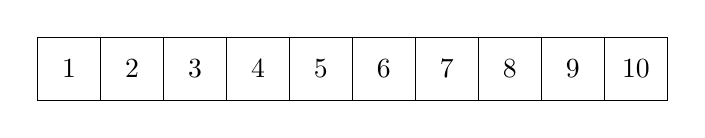
\begin{tikzpicture}
\matrix (A) [matrix of nodes, nodes={draw, minimum size=8mm},
    column sep=-\pgflinewidth]{
    1 & 2 & 3 & 4 & 5 & 6 & 7 & 8 & 9 & 10\\};
\end{tikzpicture}
\end{center}

\end{solution}

\subsection*{Problem 10}
The operation $\proc{HEAP-DELETE}(A, i)$ deletes the item in node $i$ from heap $A$. Give an implementation of $\proc{HEAP-DELETE}$ that runs in $O(\lg n)$ time for an $n$-element max-heap.
\begin{solution}
Psuedocode for heap delete: \\
\noindent
  \begin{tabularx}{\textwidth}{>{\footnotesize}rX@{}}
    \\[-1.5ex] \hline
    \multicolumn{2}{@{}l}{\refstepcounter{algorithm}\label{heap} $\proc{HEAP-DELETE}(A,i)$} \\
    \hline
     1: & \If $i > \attrib{A}{heap-size}$\\
     2: & \quad \Error $A[i]$ does not exist \\
     3: & $A[i] = A[\attrib{A}{heap-size}]$ \\
     4: & $\attrib{A}{heap-size} = \attrib{A}{heap-size} - 1$ \\
     5: & \Comment using Figure 6.2 $\proc{MAX-HEAPIFY}$ in the textbook \\
     6: & $\proc{MAX-HEAPIFY}(A, i)$ \\
\hline
  \\ [-0.2cm]
  \end{tabularx}
\end{solution}
\end{document}


